\documentclass[tikz,border=2pt]{standalone}
\usepackage{fontspec}
\setmainfont{texgyreheros}[Extension=.otf,UprightFont=*-regular,BoldFont=*-bold,ItalicFont=*-italic]
\renewcommand{\familydefault}{\rmdefault}
\usepackage{amsmath}
\usetikzlibrary{arrows.meta,calc,positioning}
\begin{document}
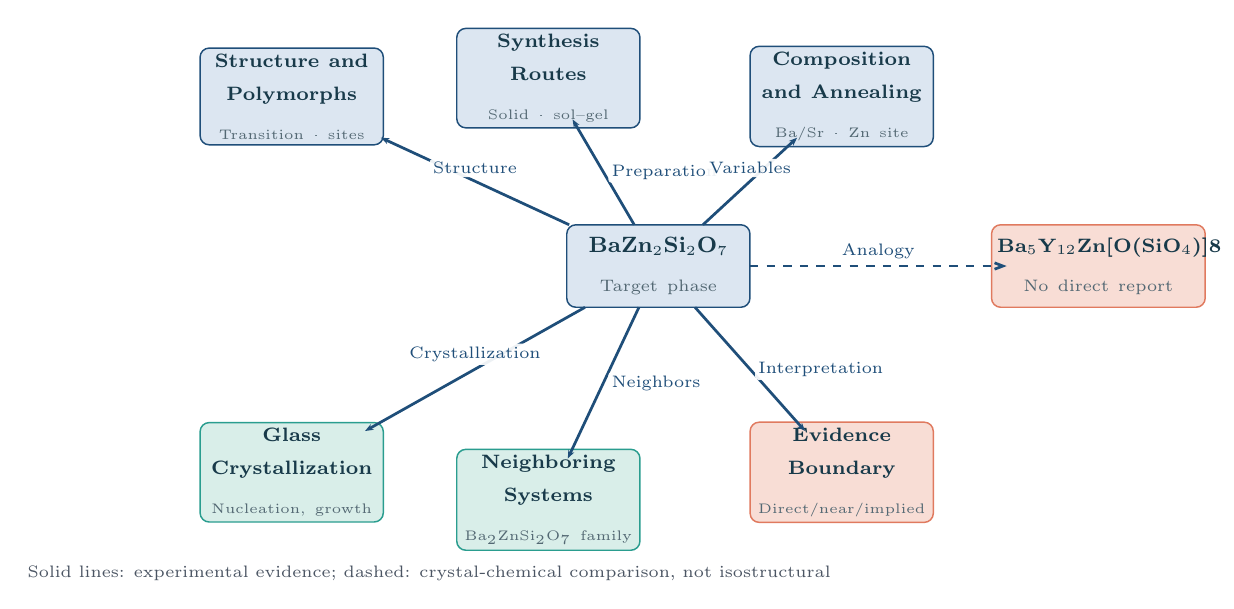
\begin{tikzpicture}[x=1pt,y=1pt, every node/.style={inner sep=0pt}]
\definecolor{nf}{HTML}{DCE6F1}\definecolor{ns}{HTML}{1f4e79}
\definecolor{lc}{HTML}{183A4A}\definecolor{sc}{HTML}{536873}
\node[draw=ns, fill=nf, line width=0.53pt, rounded corners=3.3pt, minimum width=66.2pt, minimum height=29.8pt, text width=61.2pt, align=center, inner sep=2pt, anchor=center] at (198.74pt,125.87pt) {\hyphenpenalty=9000\exhyphenpenalty=9000\relax {\bfseries\fontsize{7.6}{9.0}\selectfont\color{lc}BaZn$_{2}$Si$_{2}$O$_{7}$}\\[2.3pt]{\fontsize{6.0}{7.2}\selectfont\color{sc}Target phase}};
\definecolor{nf}{HTML}{DCE6F1}\definecolor{ns}{HTML}{1f4e79}
\definecolor{lc}{HTML}{183A4A}\definecolor{sc}{HTML}{536873}
\node[draw=ns, fill=nf, line width=0.53pt, rounded corners=3.3pt, minimum width=66.2pt, minimum height=29.8pt, text width=61.2pt, align=center, inner sep=2pt, anchor=center] at (66.25pt,187.15pt) {\hyphenpenalty=9000\exhyphenpenalty=9000\relax {\bfseries\fontsize{6.9}{8.1}\selectfont\color{lc}Structure and Polymorphs}\\[2.1pt]{\fontsize{5.4}{6.5}\selectfont\color{sc}Transition · sites}};
\definecolor{nf}{HTML}{DCE6F1}\definecolor{ns}{HTML}{1f4e79}
\definecolor{lc}{HTML}{183A4A}\definecolor{sc}{HTML}{536873}
\node[draw=ns, fill=nf, line width=0.53pt, rounded corners=3.3pt, minimum width=66.2pt, minimum height=29.8pt, text width=61.2pt, align=center, inner sep=2pt, anchor=center] at (158.99pt,193.77pt) {\hyphenpenalty=9000\exhyphenpenalty=9000\relax {\bfseries\fontsize{6.9}{8.1}\selectfont\color{lc}Synthesis Routes}\\[2.1pt]{\fontsize{5.4}{6.5}\selectfont\color{sc}Solid · sol--gel}};
\definecolor{nf}{HTML}{DCE6F1}\definecolor{ns}{HTML}{1f4e79}
\definecolor{lc}{HTML}{183A4A}\definecolor{sc}{HTML}{536873}
\node[draw=ns, fill=nf, line width=0.53pt, rounded corners=3.3pt, minimum width=66.2pt, minimum height=29.8pt, text width=61.2pt, align=center, inner sep=2pt, anchor=center] at (264.99pt,187.15pt) {\hyphenpenalty=9000\exhyphenpenalty=9000\relax {\bfseries\fontsize{6.9}{8.1}\selectfont\color{lc}Composition and Annealing}\\[2.1pt]{\fontsize{5.4}{6.5}\selectfont\color{sc}Ba/Sr · Zn site}};
\definecolor{nf}{HTML}{D9EEE9}\definecolor{ns}{HTML}{2a9d8f}
\definecolor{lc}{HTML}{183A4A}\definecolor{sc}{HTML}{536873}
\node[draw=ns, fill=nf, line width=0.53pt, rounded corners=3.3pt, minimum width=66.2pt, minimum height=29.8pt, text width=61.3pt, align=center, inner sep=2pt, anchor=center] at (66.25pt,51.34pt) {\hyphenpenalty=9000\exhyphenpenalty=9000\relax {\bfseries\fontsize{6.9}{8.1}\selectfont\color{lc}Glass Crystallization}\\[2.1pt]{\fontsize{5.4}{6.5}\selectfont\color{sc}Nucleation, growth}};
\definecolor{nf}{HTML}{D9EEE9}\definecolor{ns}{HTML}{2a9d8f}
\definecolor{lc}{HTML}{183A4A}\definecolor{sc}{HTML}{536873}
\node[draw=ns, fill=nf, line width=0.53pt, rounded corners=3.3pt, minimum width=66.2pt, minimum height=29.8pt, text width=61.2pt, align=center, inner sep=2pt, anchor=center] at (158.99pt,41.40pt) {\hyphenpenalty=9000\exhyphenpenalty=9000\relax {\bfseries\fontsize{6.9}{8.1}\selectfont\color{lc}Neighboring Systems}\\[2.1pt]{\fontsize{5.4}{6.5}\selectfont\color{sc}Ba$_{2}$ZnSi$_{2}$O$_{7}$ family}};
\definecolor{nf}{HTML}{F8DDD5}\definecolor{ns}{HTML}{e07a5f}
\definecolor{lc}{HTML}{183A4A}\definecolor{sc}{HTML}{536873}
\node[draw=ns, fill=nf, line width=0.53pt, rounded corners=3.3pt, minimum width=66.2pt, minimum height=29.8pt, text width=61.3pt, align=center, inner sep=2pt, anchor=center] at (264.99pt,51.34pt) {\hyphenpenalty=9000\exhyphenpenalty=9000\relax {\bfseries\fontsize{6.9}{8.1}\selectfont\color{lc}Evidence Boundary}\\[2.1pt]{\fontsize{5.4}{6.5}\selectfont\color{sc}Direct/near/implied}};
\definecolor{nf}{HTML}{F8DDD5}\definecolor{ns}{HTML}{e07a5f}
\definecolor{lc}{HTML}{183A4A}\definecolor{sc}{HTML}{536873}
\node[draw=ns, fill=nf, line width=0.53pt, rounded corners=3.3pt, minimum width=66.2pt, minimum height=29.8pt, text width=73.2pt, align=center, inner sep=2pt, anchor=center] at (357.74pt,125.87pt) {\hyphenpenalty=9000\exhyphenpenalty=9000\relax {\bfseries\fontsize{7.2}{8.5}\selectfont\color{lc}Ba$_{5}$Y$_{12}$Zn[O(SiO$_{4}$)]8}\\[2.2pt]{\fontsize{5.7}{6.8}\selectfont\color{sc}No direct report}};
\definecolor{ec}{HTML}{1f4e79}
\draw[draw=ec, line width=0.99pt, -{Stealth[length=3.0pt,width=2.3pt]}, rounded corners=2.0pt] (166.51pt,140.78pt) -- (98.48pt,172.24pt);
\node[fill=white, fill opacity=0.92, text opacity=1, inner sep=1.2pt, rounded corners=1pt, font=\fontsize{6.0}{6.7}\selectfont, text=ec, anchor=south, align=center] at (132.49pt,157.83pt) {Structure};
\definecolor{ec}{HTML}{1f4e79}
\draw[draw=ec, line width=0.99pt, -{Stealth[length=3.0pt,width=2.3pt]}, rounded corners=2.0pt] (190.02pt,140.78pt) -- (167.72pt,178.87pt);
\node[fill=white, fill opacity=0.92, text opacity=1, inner sep=1.2pt, rounded corners=1pt, font=\fontsize{6.0}{6.7}\selectfont, text=ec, anchor=west, align=center] at (180.52pt,159.82pt) {Preparation};
\definecolor{ec}{HTML}{1f4e79}
\draw[draw=ec, line width=0.99pt, -{Stealth[length=3.0pt,width=2.3pt]}, rounded corners=2.0pt] (214.86pt,140.78pt) -- (248.88pt,172.24pt);
\node[fill=white, fill opacity=0.92, text opacity=1, inner sep=1.2pt, rounded corners=1pt, font=\fontsize{6.0}{6.7}\selectfont, text=ec, anchor=south, align=center] at (231.87pt,157.83pt) {Variables};
\definecolor{ec}{HTML}{1f4e79}
\draw[draw=ec, line width=0.99pt, -{Stealth[length=3.0pt,width=2.3pt]}, rounded corners=2.0pt] (172.24pt,110.96pt) -- (92.75pt,66.25pt);
\node[fill=white, fill opacity=0.92, text opacity=1, inner sep=1.2pt, rounded corners=1pt, font=\fontsize{6.0}{6.7}\selectfont, text=ec, anchor=south, align=center] at (132.49pt,89.93pt) {Crystallization};
\definecolor{ec}{HTML}{1f4e79}
\draw[draw=ec, line width=0.99pt, -{Stealth[length=3.0pt,width=2.3pt]}, rounded corners=2.0pt] (191.73pt,110.96pt) -- (166.01pt,56.31pt);
\node[fill=white, fill opacity=0.92, text opacity=1, inner sep=1.2pt, rounded corners=1pt, font=\fontsize{6.0}{6.7}\selectfont, text=ec, anchor=west, align=center] at (180.52pt,83.64pt) {Neighbors};
\definecolor{ec}{HTML}{1f4e79}
\draw[draw=ec, line width=0.99pt, -{Stealth[length=3.0pt,width=2.3pt]}, rounded corners=2.0pt] (211.99pt,110.96pt) -- (251.74pt,66.25pt);
\node[fill=white, fill opacity=0.92, text opacity=1, inner sep=1.2pt, rounded corners=1pt, font=\fontsize{6.0}{6.7}\selectfont, text=ec, anchor=west, align=center] at (233.52pt,88.61pt) {Interpretation};
\definecolor{ec}{HTML}{1f4e79}
\draw[draw=ec, line width=0.99pt, -{Straight Barb[length=3.0pt,width=2.3pt]}, dashed, rounded corners=2.0pt] (231.87pt,125.87pt) -- (324.61pt,125.87pt);
\node[fill=white, fill opacity=0.92, text opacity=1, inner sep=1.2pt, rounded corners=1pt, font=\fontsize{6.0}{6.7}\selectfont, text=ec, anchor=south, align=center] at (278.24pt,127.20pt) {Analogy};
\definecolor{tc}{HTML}{4b5563}
\node[anchor=center, font=\fontsize{6.0}{7.2}\selectfont, text=tc] at (115.93pt,14.91pt) {Solid lines: experimental evidence; dashed: crystal-chemical comparison, not isostructural};
\end{tikzpicture}
\end{document}